\section{Android}

In diesem Kapitel wird das Konzept der mobilen Anwendung entwickelt. 
Das Kapitel enthält wesentliche Informationen und Schritte, die für die Entwicklung für eine Android-App erforderlich sind. 
Als Erstens wird das Konzept genau, was man in einer App-Entwicklung betrachten muss. Zweitens werden die Grundlagen vorgestellt.
Dann basierend auf dem Konzept des Projekts wird die Implementierung beschrieben.
\subsection{Mobile Apps}
Mobile Anwendungen werden unter Berücksichtigung von Faktoren wie Benutzerfreundlichkeit, Zugänglichkeit, Handbuch, Design, menschlicher Schnittstelle und Interaktion mit der Benutzererfahrung entwickelt. 
Es werden dabei unter anderem Features und Services genannt, die einen echten Mehrwert bieten und lassen die Anwendung attraktiv und innovativ erscheinen.
Über das volle Potenzial der App aufzudecken und konzeptionell zu benennen, ist wichtig, mögliche zukünftige App-Eigenschaften und -Funktionen über den Prototyp hinaus vorzuschlagen.\\
Was bei der Umsetzung der mobilen Applikation betrachten werden sollte:
\begin{itemize}
\item Die Brauchbarkeit und Nutzbarkeit 
\item Effizienz und Effektivität
\item Zuverlässigkeit
\item Saubere Interaktion
\item Dynamik und Flexibilität
\end{itemize}

\subsection{Entwicklungsumgebung: Android Studio}
Android ist das Betriebssystem und die Softwareplattform für mobile Geräte wie Smartphones
Telefone, Uhren, Fernseher oder Schnittstellen zur Kommunikation mit Fahrzeugen.
Android gehört Google und ist das am weitesten verbreitete Betriebssystem
Der weltweite Marktanteil von Smartphones liegt bei etwa 85 %.\\\\
Für die Entwicklung von Android Apps kann Android Studio verwendet werden. 
Es bezieht sich auf die offizielle integrierte Entwicklungsumgebung (IDE) für Android. Die IDE hilft beim Entwerfen und Entwickeln Android-Anwendungen mit vielen Hilfsfunktionen. Es hat gute integriertes Support-Capability-Management für Gradle, die Software für Android-Apps verwendete Build-System. Neue Abhängigkeiten sind normalerweise direkt unter verfügbar Quellcode-Editor, keine Notwendigkeit, Build-Skripte manuell zu bearbeiten. 
Android Studio hat auch viele andere sehr nützliche Funktionen, die oben nicht aufgeführt sind, wie z. B. eine integrierte Software-Versionskontrolle, effektive Debugging-Tools und einen sehr intelligenten Code-Inspektor\cite{AndSt}.
\subsection{Flutter}
Was ist Flutter? Flutter ist ein von Google entwickeltes Framework um nativ kompilierbare Anwendungen anhand einer einzigen Codebasis zu schreiben.
Flutter ist ein Open-Source-Framework von Google zur Entwicklung grafischer Anwendungen, die auf Mobilgeräten, Browsern und Computern ausgeführt werden. Der wichtige Aspekt sind die verschiedenen gemeinsamen Codebasen
Plattform und laufen mit nativer Geschwindigkeit. Die gleiche Anwendung kann also auch ohne viele Änderungen auf eine andere Plattform kompiliert werden. Flutter bietet umfangreiche Bibliotheken mit vorgefertigten UI-Elementen.Datenströme sind sehr einfach zu implementieren und stellen sicher, dass Benutzer immer auf dem neuesten Stand sind.\\
Die Verwendung des Flutter-Frameworks bietet mehrere Vorteile. Wie bereits erwähnt, liegt ein besonderer Fokus darauf, eine einzige Codebasis für viele Menschen zu verwenden Tree Form aufbauen. Das spart im Idealfall Zeit und Geld. Mit der “Hot Reload“ Funktion ermöglicht es Entwicklern, schnell und einfach Schnittstellen zu erstellen, neue Funktionen hinzuzufügen und  
Fehler schneller finden\cite{Flut}.
\subsection{Dart}
Flutter läuft auf Dart, der hauseigenen Programmiersprache von Google und basiert darauf.
Dart ist eine von Google entwickelte Computersprache. Sein ursprüngliches Ziel war es, JavaScript zu ersetzen und die neue Sprache zu werden
ein Netzwerk werden. Ihr derzeitiger Fokus liegt jedoch mehr auf JavaScript.
Der Code zum Konvertieren und über die Entwicklung von Multi-Plattform-Programmen.\\
Die Eigenschaften von Dart sind:
\begin{itemize}
\item Eine leichte zu lernende Sprache
\item Eine Gute Dokumentation
\item Eine hoher Leistungsfaktor
\item Eine klare und saubere Syntax
\item Hat unglaubliche Tools zur Unterstützung der App-Entwicklung
\end{itemize}
\subsection{Konzept: SchrödingerSAlarm}
Beim Projekt ist die Mobile Android app ein Wichtig Bauteil des Systems.
die Mobile App soll wie eine gewöhnliche Android App. Die App soll für jedes Android Smartphone kompatibel sein. Um mehr die Funktionalität der App wird durch die beiden Abbildungen dargestellt:\\
\textbf{Standard Fall:} Die App ist mit dem Webserver verbunden. Alle Informationen. die vom Webserver kommen, werden in der App angezeigt. Die Koordinaten sollen den Standort des Automobilfahrzeug auf einer Karte in der App angezeigt werden.
\begin{figure}[H]
            \centering
            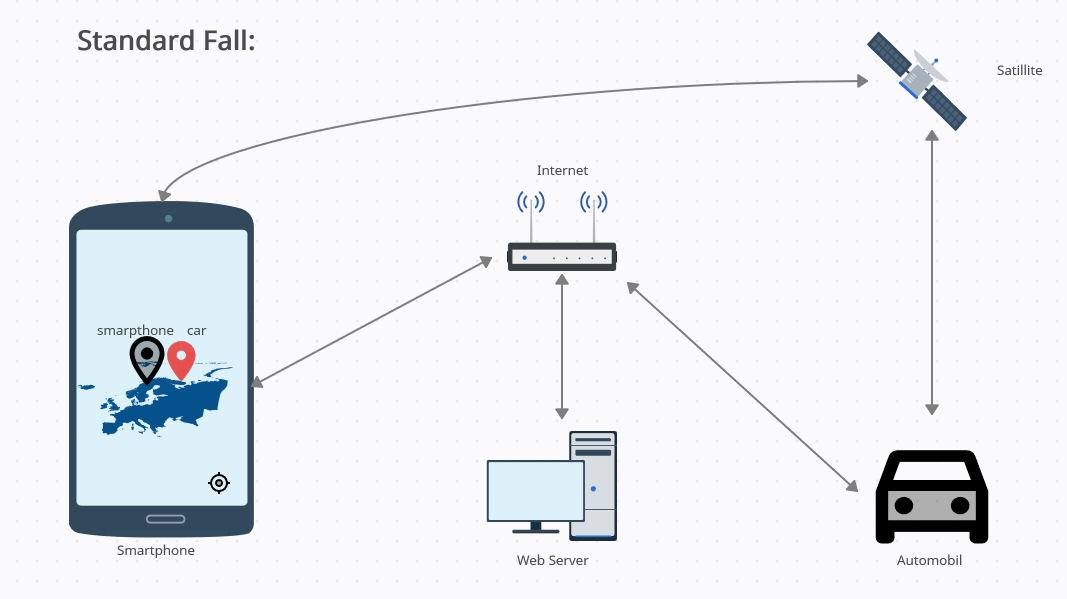
\includegraphics[width=1\textwidth]{Bilder/StandardFall.PNG}
            \caption{Konzept der Android App im AlarmFall}
\end{figure}
\textbf{Alarm Fall:} Im Falle das der Standort des Automobils sich bewegt und das Standort des Smartphones konstant ist, wird ein Alarm auf dem Handy ausgelöst und der Nutzer bekommt eine Push-Benachrichtigung.
     \begin{figure}[H]
            \centering
            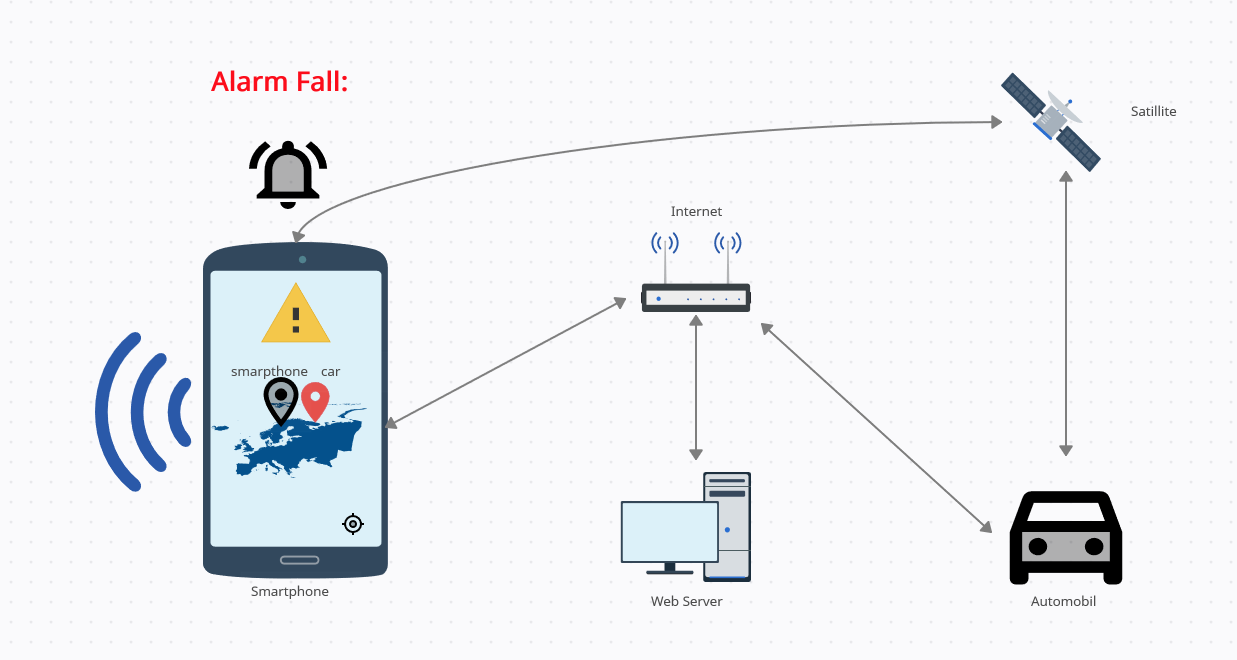
\includegraphics[width=1\textwidth]{Bilder/AlarmFall.PNG}
            \caption{Konzept der Android App im Standard Fall}
	
    \end{figure}
	
\subsection{Implementierung}
\subsubsection{Flutter Funktionalität}
Flutter ist sehr einfach zu verstehen und verkürzt die Lernkurve erheblich. Die Grundidee lautet: “Alles ist ein Widget“. Es ist dem Entwickler völlig selbst uberlassen wie er sein Projekt
strukturieren und hinsichtlich Architektur- und Entwurfsmuster logisch aufbauen möchte. Der Einstiegspunkt zu Flutter ist die main.dart-Datei oder die zentrale main()-Methode. Von dort aus ist es möglich, sich gegenseitig zu verschachteln und zu importieren. 
Die Entwicklung von Flutter beinhaltet hauptsächlich nur Widgets, weil alles hineingeschrieben wird.
Sogar ein einfacher Text “Teil“ wird als Widget festgelegt. 
\\
In Flutter gibt es wieder eine Baumstruktur “Widget Tree“. Jede betriebssystemspezifische Komponente, die man in Flutter verwenden möchte, muss zunächst von einem Flutter-Entwickler nativ entwickelt werden. Dies ist jedoch nur dann erforderlich, wenn die Anwendung auch der nativen Anwendung ähnlich sein soll. 
Aus den Basis-Komponenten aus den verschiedenen Paketen konnte man eigene Widgets schreiben. So kann sich ein eigener, abgerundeter Button beispielsweise durch eine Kombination aus RawMaterialButton, Text und Icon-Widgets darstellen lassen.
In Flattern werden Widgets jedoch als einfache Klassenvariablen über den Konstruktor der Klasse übergeben und können dort beliebig verwendet werden.
Durch die Klassenvariablen lassen sich Komponenten in
ihrem Aussehen sowie ihrer Funktionalität individualisieren und anpassen \cite{SDK}.\\
Es gibt zwei Arten von Komponenten in Flutter, die im Code explizit als solche benannt werden. Erstens ist es “Statful-Widgets“, die einen Zustand beibehalten oder verwalten können. Andererseits gibt es “Stateless Widgets“, die nur als statische, einfache Widgets dienen. Ein zustandsbehaftetes Widget erfordert immer eine zugeordnete createState()-Funktion. Eine Methode, die ein Zustandsobjekt (private Klasse) erstellt, das wiederum
verwaltet den Widget-Status. Abgesetzt durch Aufruf von setState ()
ruft die Methode build() auf, um die Komponente neu zu zeichnen. Die Methode build() wird beim Casting von Stateless verwendet
Ausgelagerte Widgets an das State-Widget in der privaten State-Klasse.\\
Das Styling in Flutter ist grundlegend speziell. Da alles ein Widget ist, so auch die Design Möglichkeiten realisiert.
Wenn man das Widget zentrieren möchten, könnte man beispielsweise das Center-Widget verwenden.
Um ein Widget von anderen Widgets entfernen möchte, muss dafür mit einem Padding-Widget umschlossen werden. Einfaches Beispiel in Text-Widget wird von einem zentralen Widget umgeben, das folgt
es ist wiederum vom Container-Widget umhüllt.\\\\
“Center“, “Raw“, “Column“, “Container“-Widgets und viele andere Widgets
sind die Bausteine in der Entwickelung von Flutter App.
\subsection{Implementierung SchrödingersAlarm App}
\subsubsection{Login Menü}
Das Starten der App ist hier Standard, wie eine jede App. Zuerst die Willkommensseite, in der soll ein Login Menü erscheinen. 
Jedes Gerät soll eine eigene IMEI und der PIN Code haben und den Kunden mitgeliefert. 
Diese beiden Informationen sind in der Datenbank auf der App eingefügt. Die Login-Seite beinhaltet zwei Komponenten.
Das Logo des Produkts wird oben direkt angezeigt. Unten sind zwei Eingabefeldern definiert,
in der man die Login-Informationen(IMEI/PIN) eingeben kann. Natürlich wird ein “Einloggen“ Button unter den Feldern gesetzt.
Der Login-Prozess hat ein genau definierten Mechanismus. In den beiden Feldern muss eine bestimmte Anzahl eingegeben werden. Ansonsten wird es nicht akzeptiert. Die IMEI muss 15 Ziffern beinhalten.  Die PIN code muss 6 Ziffern beinhalten.  Nur bei einer korrekten Dateneingabe wird man in der nächsten Seite geleitet.
Andernfalls erschient eine rote Fehlermeldung, die um korrekte Informationen bittet.\\\\
Die Umsetzung in Flutter ist simpel gestellt. Ein Widget wird als gesamte Seite implementiert. 
Wie vorher beschrieben ist, wird horizontale aufgeteilt. Der obere Teil ist das importierte Bild vom LOGO und der untere Teil von den Eingabefeldern. 
Diese Aufteilung wird mit einem “Column“ Widgets definiert. Der unter Teil wird auch in viele Widgets aufgeteilt. 
Darunter sind zwei Eingabefeldern und der “Einloggen“ Button.
 \begin{figure}[H]
            \centering
            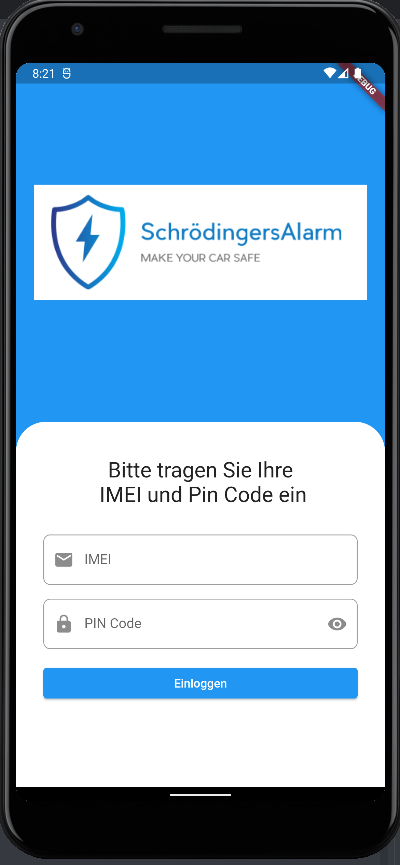
\includegraphics[width=0.5\textwidth]{Bilder/LoginIn.PNG}
            \caption{Android App: Login Seite}
    \end{figure}

\subsubsection{Hauptseite}
Nach erfolgreichem Login leitet die App den Nutzer auf der Hauptseite.
Auf der Hauptseite gibt es einer horizentalen Appbar von 3 Kategorien (Home/Status/Maps), links oben ein Menu item für Support und rechts oben ein logout item für das Ausloggen aus der App. 
Im Home wird das Logo und Standpunkt der aktuellen Lage angezeigt.
Wenn das Auto sicher gemeldet ist, wird ein grüner Kreis mit der Meldung “your car is safe“ angezeigt. 
Falls das Auto nicht im sicheren Zustand ist, wird ein roter Kreis mit der Meldung “Dangerous situation“.\\\\
Durch das Drücken auf „Status“ in der horizentalen Appbar, werden die Informationen, die aus dem Webserver kommen, in einem Text Widget angezeigt.
Wichtig hier ist auf eine Webserver Verbindung zu prüfen. Falls es eine Verbindung gibt, soll ein Grüne Verbindung Icon angezeigt werden.
Im Falle einer Störung wird ein Icon “nicht verbunden“ angezeigt.\\\\
Das dritte Item in der horizontalen Appbar ist die Karte. In der wird die Google Maps Anwendung in der App geöffnet.
Die Koordinaten, die von dem Webserver kommen, werden dann in einem Marker in der Google Maps Karte markiert. 
Dazu kommt der aktuelle Standort des Smartphones über den GPS in einem andren Marker angezeigt.\\\\
Falls die Koordinaten vom Webserver weit entfernt von den interpretierten Koordinaten vom GPS Smartphones ist, bekommt man eine Push-Benachrichtigung. Bei der Umrechnung werden Longtitude und Latitude von beiden Koordinaten abgezogen und den Beitrag von den beiden Werten gerechnet. 
Falls einer der beiden Werten höher als der festgelegten Wert ist, wird die App eine Push-Benachrichtigung erstellt.
 	\begin{figure}[H]
   \centering
            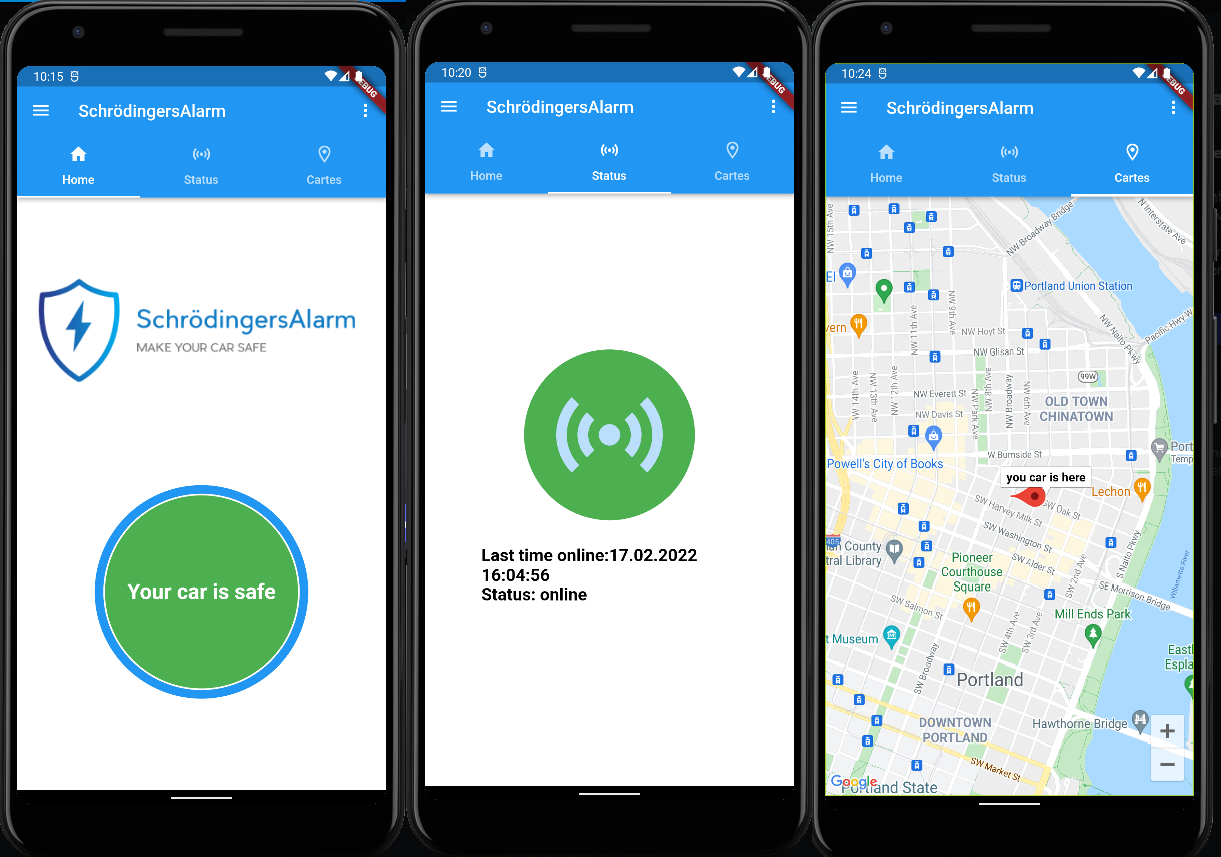
\includegraphics[width=0.75\textwidth]{Bilder/hauptseite.PNG}
		            \caption{Android App: Hauptseite}
    \end{figure}
